\section{Adaptation results}

After implementing the parameter changes described in Section \ref{sec:adaptations} we ran the comprehensive test of 3600 sessions again, with the \emph{differences} in the results showing the following graphs.

\subsection{Difference in Amount of Agreements}

Looking at Figure \ref{fig:post_18_agreements} and \ref{fig:post_180_agreements}, we see that the short negotiations are less likely to end in an agreement. In contrast to the long negotiations, where there is no observable difference. This is very likely the result of our now less sensitive parameters.

\begin{figure}[H]
	\minipage{0.49\textwidth}
	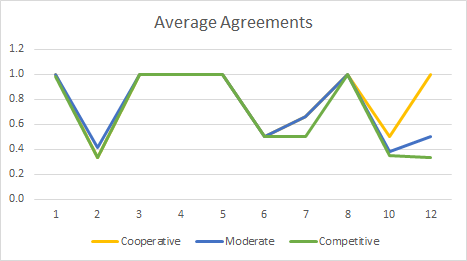
\includegraphics[width=\linewidth]{post/18_agreements}
	\caption{18 Rounds per Opponent}
	\label{fig:post_18_agreements}
	\endminipage\hfill
	\minipage{0.49\textwidth}
	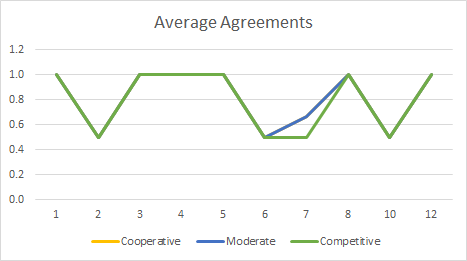
\includegraphics[width=\linewidth]{post/180_agreements}
	\caption{180 Rounds per Opponent}
	\label{fig:post_180_agreements}
	\endminipage\hfill
\end{figure}

\subsection{Difference in Distances to Nash and Pareto}

Seen from Figure \ref{fig:post_18_distance_nash} \ref{fig:post_180_distance_nash}, \ref{fig:post_18_distance_pareto} and \ref{fig:post_180_distance_pareto}, we see a little fluctuation around the 0-axis, with the occasional spike. The overall trend is a lower distance, with the exception of Opponent 7. This opponent has bigger distances in the shorter negotiations. These results indicate a slightly better negotiation strategy after the changes made.

\begin{figure}[H]
	\minipage{0.49\textwidth}
	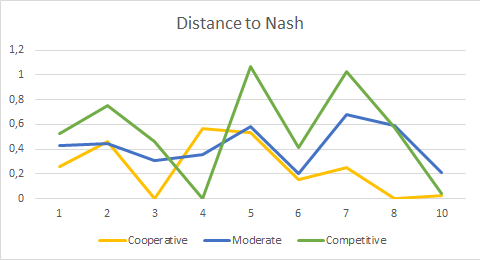
\includegraphics[width=\linewidth]{post/18_distance_nash}
	\caption{18 Rounds per Opponent}
	\label{fig:post_18_distance_nash}
	\endminipage\hfill
	\minipage{0.49\textwidth}
	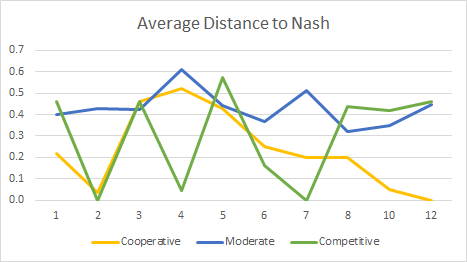
\includegraphics[width=\linewidth]{post/180_distance_nash}
	\caption{180 Rounds per Opponent}
	\label{fig:post_180_distance_nash}
	\endminipage\hfill
\end{figure}

\begin{figure}[H]
	\minipage{0.49\textwidth}
	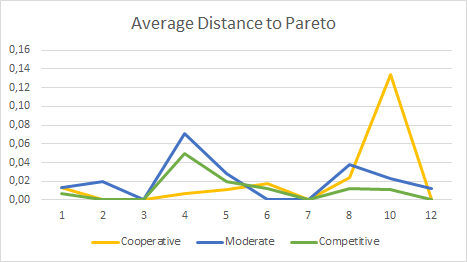
\includegraphics[width=\linewidth]{post/18_distance_pareto}
	\caption{18 Rounds per Opponent}
	\label{fig:post_18_distance_pareto}
	\endminipage\hfill
	\minipage{0.49\textwidth}
	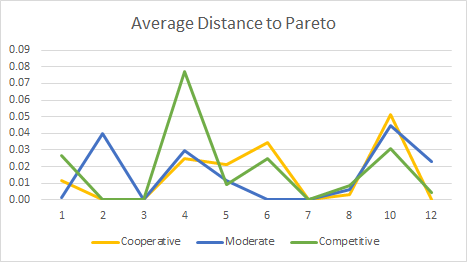
\includegraphics[width=\linewidth]{post/180_distance_pareto}
	\caption{180 Rounds per Opponent}
	\label{fig:post_180_distance_pareto}
	\endminipage\hfill
\end{figure}

\subsection{Difference in Social Welfare}

Figure \ref{fig:post_18_social_welfare} and \ref{fig:post_180_social_welfare} show good news all around for the differences in Social Welfare! With the small exception for Opponent 7 in the short negotiations and opponent 10 in the long negotiations, we see a significant positive change in social welfare after the made changes.

\begin{figure}[H]
	\minipage{0.49\textwidth}
	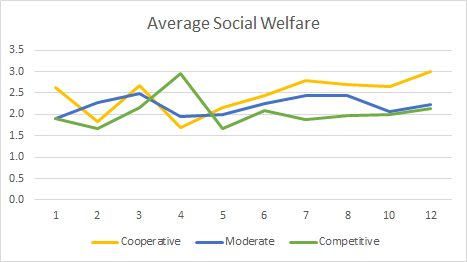
\includegraphics[width=\linewidth]{post/18_social_welfare}
	\caption{18 Rounds per Opponent}
	\label{fig:post_18_social_welfare}
	\endminipage\hfill
	\minipage{0.49\textwidth}
	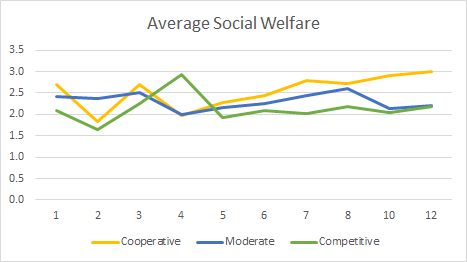
\includegraphics[width=\linewidth]{post/180_social_welfare}
	\caption{180 Rounds per Opponent}
	\label{fig:post_180_social_welfare}
	\endminipage\hfill
\end{figure}

\subsection{Difference in Cooperative Utilities}

As shown in Figure \ref{fig:post_18_utils_domain_cooperative} and \ref{fig:post_180_utils_domain_cooperative}, it is clear that there is a significant improvement in our utilities for the cooperative domain.

\begin{figure}[H]
	\minipage{0.49\textwidth}
	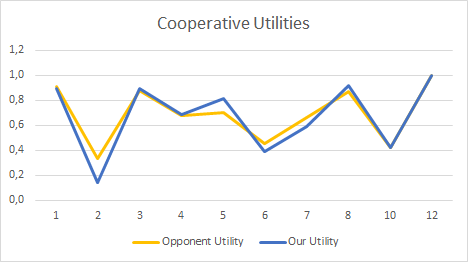
\includegraphics[width=\linewidth]{post/18_utils_domain_cooperative}
	\caption{18 Rounds per Opponent}
	\label{fig:post_18_utils_domain_cooperative}
	\endminipage\hfill
	\minipage{0.49\textwidth}
	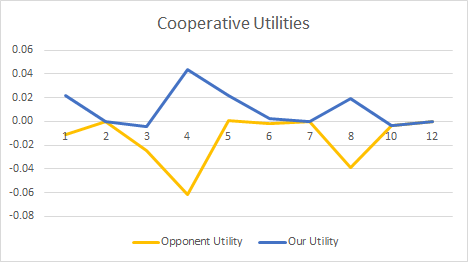
\includegraphics[width=\linewidth]{post/180_utils_domain_cooperative}
	\caption{180 Rounds per Opponent}
	\label{fig:post_180_utils_domain_cooperative}
	\endminipage\hfill
\end{figure}

\subsection{Difference in Moderate Utilities}

Figure \ref{fig:post_18_utils_domain_moderate} and \ref{fig:post_180_utils_domain_moderate} also show a significant improvement in our performance for the moderate domain.

\begin{figure}[H]
	\minipage{0.49\textwidth}
	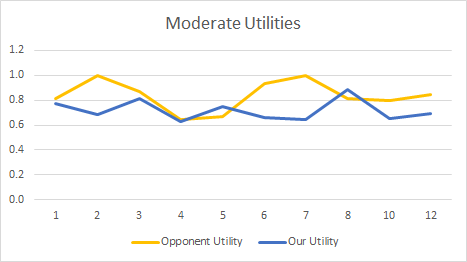
\includegraphics[width=\linewidth]{post/18_utils_domain_moderate}
	\caption{18 Rounds per Opponent}
	\label{fig:post_18_utils_domain_moderate}
	\endminipage\hfill
	\minipage{0.49\textwidth}
	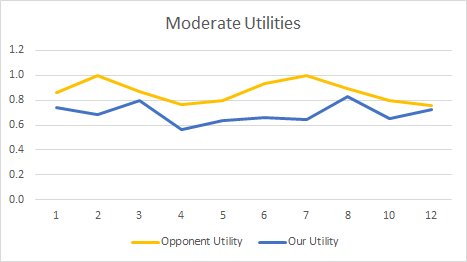
\includegraphics[width=\linewidth]{post/180_utils_domain_moderate}
	\caption{180 Rounds per Opponent}
	\label{fig:post_180_utils_domain_moderate}
	\endminipage\hfill
\end{figure}

\subsection{Difference in Competitive Utilities}

Lastly, for the competitive domain, Figure \ref{fig:post_18_utils_domain_competitive} and \ref{fig:post_180_utils_domain_competitive} also show a significant improvement in our final average utility.

\begin{figure}[H]
	\minipage{0.49\textwidth}
	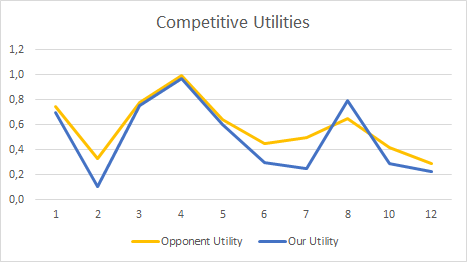
\includegraphics[width=\linewidth]{post/18_utils_domain_competitive}
	\caption{18 Rounds per Opponent}
	\label{fig:post_18_utils_domain_competitive}
	\endminipage\hfill
	\minipage{0.49\textwidth}
	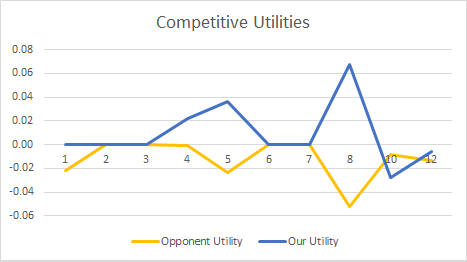
\includegraphics[width=\linewidth]{post/180_utils_domain_competitive}
	\caption{180 Rounds per Opponent}
	\label{fig:post_180_utils_domain_competitive}
	\endminipage\hfill
\end{figure}